\subsubsection*{ --- Integration}\par
With the design of the mechanical, electrical, computational/software systems happening concurrently, it all needs to eventually be integrated to make the entire project work according to the target specifications.\par
\vspace{.167in}
\noindent\underline{Electrical to Mechanical system:}\par
\vspace{.08in}
Firstly for the load cell, it would be the design on how the load cell will be mounted to allow it to detect human force input in the desired direction, and how to pre-load the load cell in order to allow it to sense forces in two-directions. This resulted with the design of the cart and handle, its metal plate braces and using the M10 bolt to pre-load the load cell.\par
Secondly for the motor, it would be the design on how to mount the motor to be at the right height when pulling the cart and how the cart will hit the limit switches at the either end of the track. This resulted with the design of the motor mount and the limit stops.\par
\vspace{.167in}
\noindent\underline{Computational/Software to Electrical system:} \par
\vspace{.08in}
The interaction between the software and the electrical system is the most crucial interaction that must be integrated in the design of the project. This is because most of the mechanical actuation or sensing in the project will always pass through this phase. For example, the load cell must be calibrated in order for the controller to know the amount of force input by the operator, and the encoder must also be calibrated in order to obtain the correct velocity. \par
\begin{figure}[ht]
\begin{center}
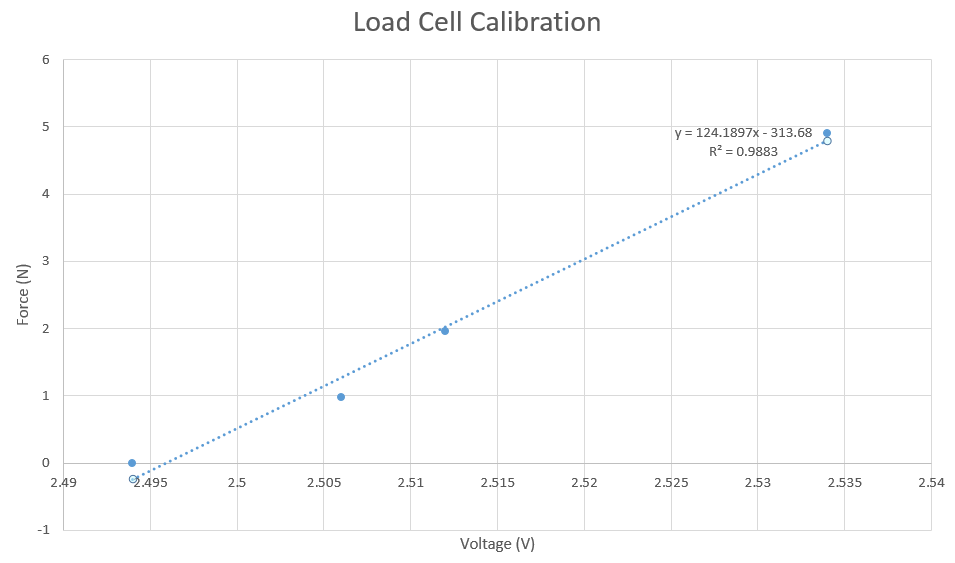
\includegraphics[width=2.75in]{Images/load_cell_cali.PNG}
\caption{Load Cell Calibration Plot}
\label{LC_cali}
\end{center}
\end{figure}
The calibration of the load cell is done by testing its voltage output using a known mass, then the data points are plotted in Figure \ref{LC_cali} and the linear fit coefficients found are implemented into the C code to convert voltage to force reading.\par
The calibration of the encoder is done by using equation \ref{Veq}:
\begin{equation}
\label{Veq}
    Vel=(\frac{BDI}{BTI})(\frac{1 rev}{2048 BDI})(\frac{BTI}{5 ms})(\frac{1000 ms}{s})(\frac{1}{5.9})(\pi)(0.01834 m)
\end{equation}